\section{Introduction}

In the "Design Principles for Precision Mechanisms II" course a project has to be made. The project is provided by DEMCON, a spin off of the University of Twente. DEMCON is a company which develops and produces systems, with as focus areas high-tech, medical, optomechatronic, robotic and industrial systems $\&$ vision.

The project is based on the Nanomefos system, a 5 DOF machine which measures the form of freeform optics  of aspheric lenses. The goal is to design a miniature version of the Nanomefos which can be used in the production of lenses for smartphone cameras and small microscopes. Three types of concepts have to be developed: one concept with conventional joints, one with only flexures and a combined flexure. 

In this report first the problem is analysed in the problem statement, which is stated below, resulting in
requirements and assumptions about the problem. In the concepts part a few ideas are presented to solve
the problem. The best suitable option is chosen and further developed in the final design part.

\begin{figure}[h]
    \centering
    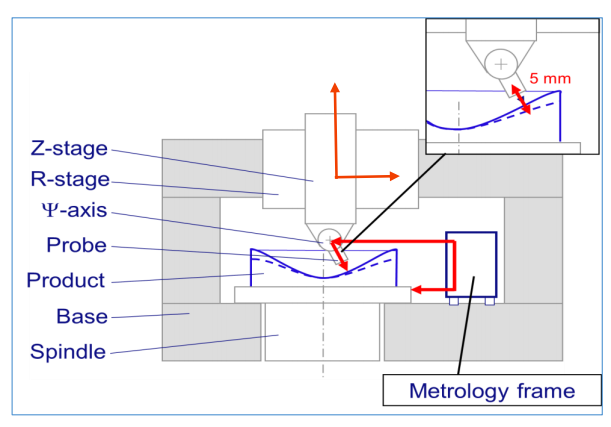
\includegraphics[width=0.6\textwidth]{images/Nanomefos.png}
    \caption{An overview of the current Nanomefos system}
    \label{fig:Nanomefos}
\end{figure}

\subsection{Problem statement}


\subsection{Requirements and Assumptions} \label{sec:requirements}
\label{requirementandassumptions}
To obtain a good design for the miniature version of the Nanomefos a number of requirements and assumptions has been made. 

\subsubsection*{Requirements}
The total mass of the probe should be $\leq 0.5\ kg$, furthermore the total space which the systems occupies has to be $\leq 300\cdot300\cdot100\ mm$.

In table \ref{tab:requirements} an overview is given of the range, duration, repeatability, velocity and acceleration for each degree of freedom. Both the range, duration and repeatability where given. Whereas the maximum velocities and accelerations are determined. 

The system has the following degrees of freedom: a translation in the x direction with a stroke of 10 mm, a translation in the z direction with a total stoke of 2 mm, a rotation around the y axis of 45 degrees and a rotation around the z axis of 90 degrees. An overview of the degrees of freedom is shown in table \ref{tab:doftable}.
\begin{table}[!h]
\centering
\caption{Required range of motion per degree of freedom}
\label{tab:doftable}
\begin{tabular}{l|llll}
Degree of Freedom & X-translation & Z-translation & Y-rotation & Z-rotation \\ \cline{1-5}
Range of motion   & 10 mm         & 2 mm          & 45 \degree  & 90 \degree 
\end{tabular}
\end{table}

\subsubsection*{Derivation of maximum velocities and accelerations}
To determine the maximum velocities and accelerations for all four degrees of freedom (X, Z, $R_y$, $R_z$), a skew sine function has been assumed for the position of the probe. This can bee seen in equation \ref{eq:skewsine}, where $h_m$ is the range of the desired displacement/rotation of the degree of freedom, while $t_m$ is the time needed to achieve this displacement/rotation.

\begin{equation} \label{eq:skewsine}
r(t)=\frac{h_m}{t_m}t-\frac{h_m}{2\pi}\sin\left(\frac{2\pi}{t_m}t\right) \\
\end{equation}

Using equation \ref{eq:skewsine}, and taking the derivative, the velocity, acceleration and jerk can be determined as seen in equation \ref{eq:skewsinederivative}. 
\begin{equation} \label{eq:skewsinederivative}
\begin{aligned}
v(t)=&r'(t)=\frac{h_m}{t_m}-\frac{h_m}{t_m}\cos\left(\frac{2\pi}{t_m}t\right) \\ 
a(t)=&r''(t)=\frac{2\pi h_m}{t_m^2}\sin\left(\frac{2\pi}{t_m}t\right) \\ 
J(t)=&r'''(t)=\frac{4\pi^2h_m}{t_m^3}\cos\left(\frac{2\pi}{t_m}t\right)
\end{aligned}
\end{equation}
The maximum velocity occurs at $a(t)=0$, while the maximum acceleration occurs at $J(T)=0$. When solving these equations for t, the time at which the maxima occur are found. Plugging this back into the original velocity and acceleration equation, the results are obtained. This can be seen in equation \ref{eq:VmaxAmax}
\begin{equation} \label{eq:VmaxAmax}
\begin{aligned}
\text{Determination of $v_{max}$} \Rightarrow \quad a(t)=0 \Rightarrow \quad t=\frac{t_m}{2} \quad \quad \quad \quad  \quad \quad & v_{max}=r'\left(\frac{t_m}{2}\right)=\frac{2h_m}{t_m} \\
\text{Determination of $a_{max}$} \Rightarrow \quad J(t)=0 \Rightarrow \quad t=\frac{t_m}{4} \quad \quad \quad \quad  \quad \quad & a_{max}=r''\left(\frac{t_m}{4}\right)=\frac{2\pi h_m}{t_m^2}
\end{aligned}
\end{equation}
Using the final expressions for the maximum velocities and accelerations, the values for all four degrees of freedom are calculated, which can be seen in table \ref{tab:requirements}.
\begin{table}[ht]
\centering
\caption{Range, duration, repeatability, velocity and acceleration per degree of freedom}
\label{tab:requirements}
\begin{tabular}{l|lllll}
\textbf{DoF} & \textbf{Range ($h_m$)}    & \textbf{Duration ($t_m$)} 	& \textbf{Repeatability} & \textbf{Velocity ($v_{max}$)} & \textbf{Acceleration ($a_{max}$)} \\ \hline
$X$                & $ \geq \pm \ 5 mm $ 		& 0.5 s 						& $\leq 1\ \mu m$         & $ 40\ mm/s $        & $  125\ mm/s^2 $                    \\
$Z$                & $ \geq \pm \ 1 mm$  		& 0.5 s						& $\leq 1\ \mu m$            &$  8\ mm/s $       &  $ 25\ mm/s^2 $                    \\
$R_y$              & $ \geq 0.785\ rad $       & 2.0 s							& $\leq 10\ \mu rad$         & $ 0.79\ rad/s$  &   $  1.23\ rad/s^2 $                \\
$R_z$              & $ \geq  1.571 \ rad $     		& 1.0	s				    & $\leq 10\ \mu rad$         & $ 3.14\ rad/s $ &   $  9.87\ rad/s^2$                 
\end{tabular}
\end{table}

\subsubsection*{Eigenfrequencies}
The internal parasitic eigenfrequency should be $\geq 200\ Hz$. To obtain the minimum lowest mechanical natural frequency the crossover frequency should be multiplied by a factor 4.

\subsubsection*{Assumptions}
To obtain a design for the miniature version of the Nanomefos a number of assumptions has been made shown in 


%\subsection{Sequence of DOF}
%As mentioned in section \ref{requirementandassumptions} there are two translational degrees of freedom and two rotational degrees of freedom. These DOF's need to be positioned in series to achieve the required range of motion. The sequence in which the DOF's are positioned in series influence the stiffness and the range of motion significantly, therefore an evaluation is done to determine the best sequence.

%\begin{wrapfigure}{r}{0.5\textwidth}
%  \begin{center}
%    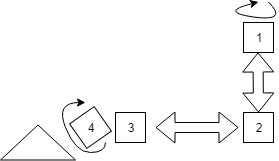
\includegraphics[width=0.4\textwidth]{images/DOF_sequence.png}
%  \end{center}
%  \caption{Sequence of DOF's}
%  \label{fig:sequencedof}
%\end{wrapfigure}

%The sequence of DOF's is visualized in figure \ref{fig:sequencedof}. Step 1 is the z-rotation of 90\degree, this has to be done first to achieve the half circle range of motion with as little required space as possible. Then in step 2 the probe is positioned at the correct height by the 2 mm of z-translation after which it is translated in the x-direction to get to its final position. As can be seen in the figure the surface of the disk is under an angle, therefore the probe will then be rotated around it's y-axis to achieve the correct orientation. 
